 \section{Methodology}\label{sec:methodology}
Prevalence of large organizations owning multiple ASes, the widespread use of CDN, multinational organizations make it difficult to separate malicious hijacks from non-malicious ones. In this section, we present our algorithm for filtering out AS origin-conflict events that are most likely not a hijack. Lack of ground truth except for manually browsing the internet makes it difficult to evaluated the effectiveness of our algorithm. Our goal for our algorithm is for it to be able identify hijacks with a high probability and in real time.\\
To identify as AS-origin conflicts, we analyzed the BGPStream data from the first hour of every day for the month of April, 2017. Average size of a Routing table is around 512K and combining that with frequent updates and multiple collecters makes the size of data available via BGPStream very large\cite{noauthor_bgp_nodate}. We choose the month of April to sample our data from because BGPStream twitter account showed  a large number of hijacks occurring in this month.\\To get information about AS peering relationships and AS to organization name mapping, we used the data sets available via CAIDA\cite{mapping}. We chose python to code our algorithm given the ease of data parsing in python.\\ 
Figure~\ref{fig:flowchart} presents a high level flowchart of our algorithm.
 \begin{figure}[!htbp]
	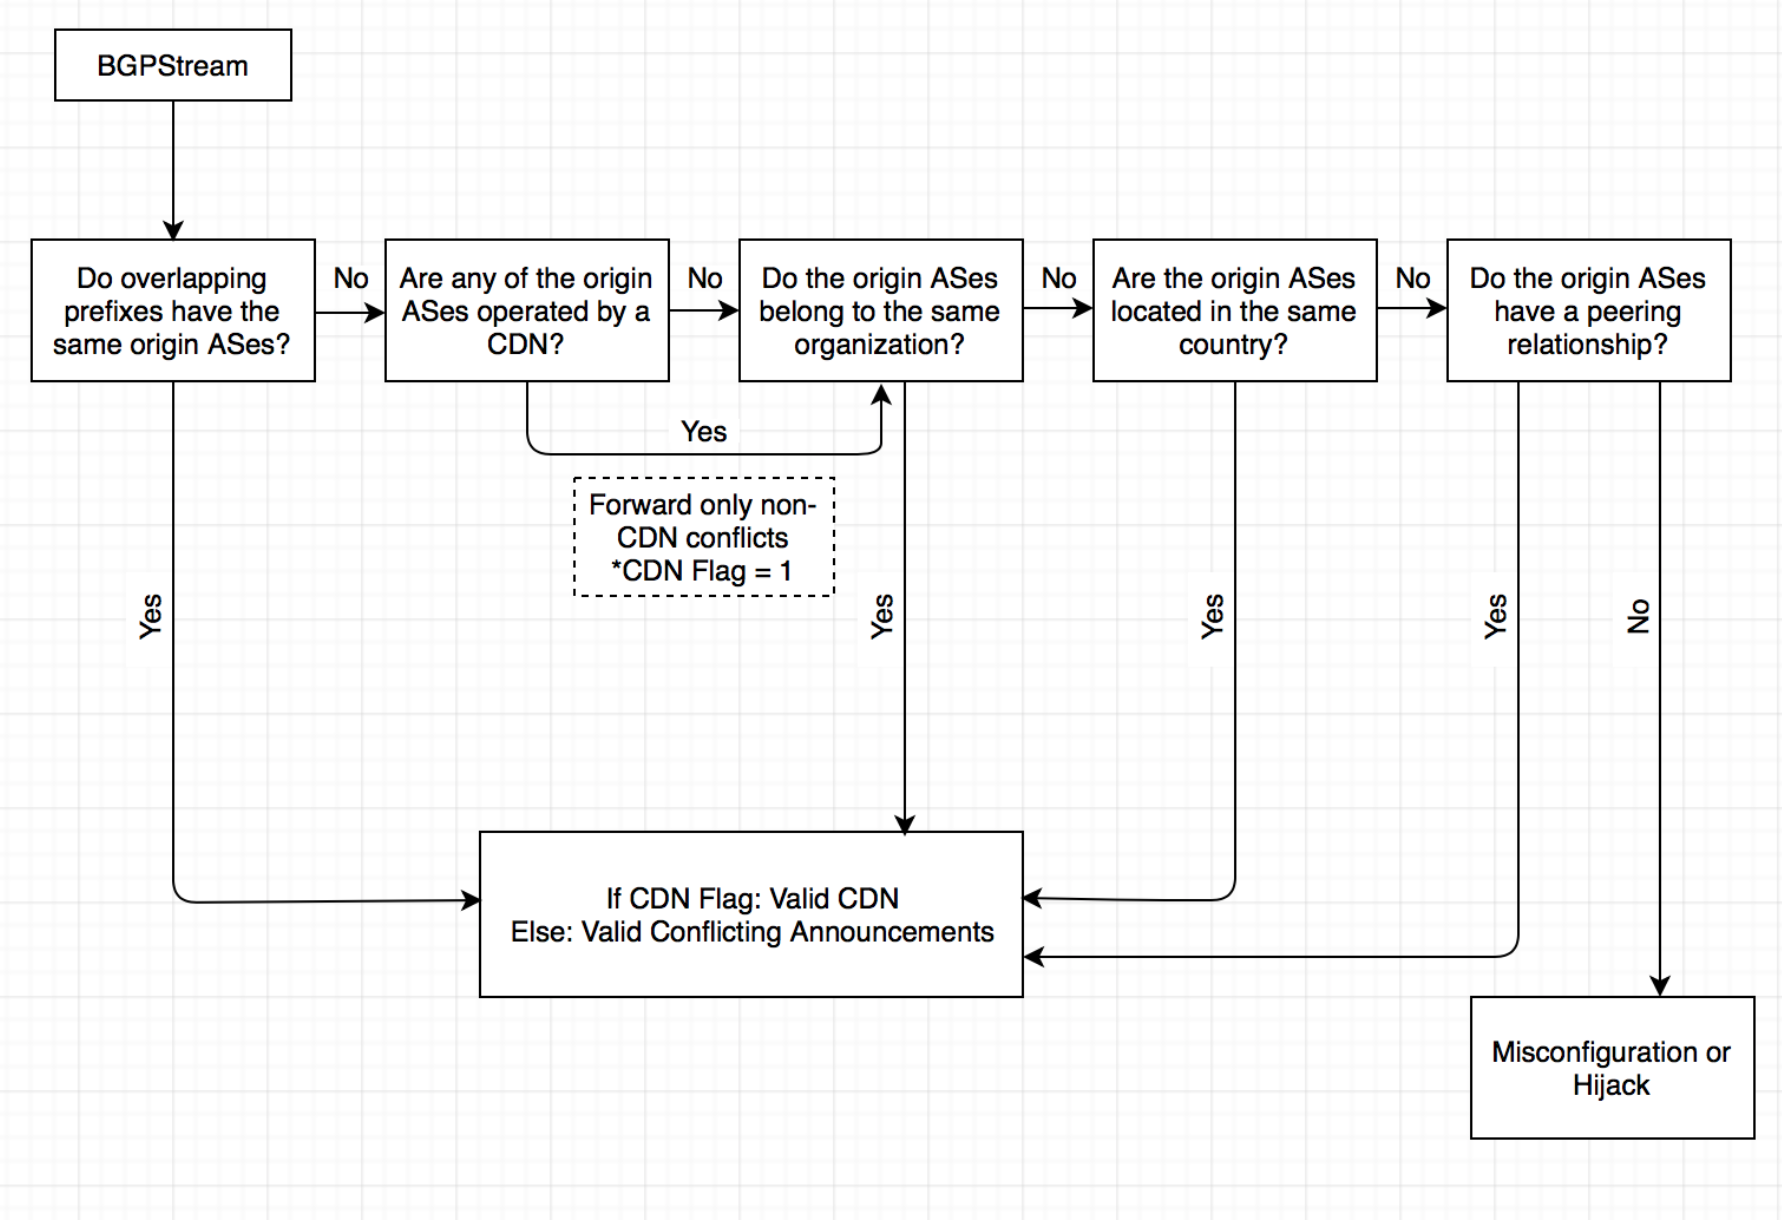
\includegraphics[width=0.5\textwidth]{flow.png}
	\caption{Our algorithm flow chart through which AS-origin conflicts were categorized using BGPStream and CAIDA.}
	\label{fig:flowchart}
\end{figure}

\subsection{Algorithm for Identifying Source of Conflicts}
Identifying the reason of origin AS conflicts involves carefully filtering RIB table records. Here, we describe our method of filtering possibly non-malicious conflicts. 
\begin{enumerate}
\item The first step is identifying the instances where we saw two different ASes announcing the same BGP prefix/es. We took the data set we got from BGPStream and identified all instances where a prefix or a more-specific prefix than previously found was being announced by different origin ASes. 
\item We use CAIDA AS information to check if any of the origin ASes owner is a CDN\cite{mapping}. To identify a CDN, we used regular expression matching between the AS owner's organization name and a list of most popular CDNS that we got from the internet. CDNs may announce the same prefix in different parts of the world for traffic engineering. This lead to clients being directed to the closest CDN cache. If any AS is operated by a CDN, we set a flag, noting the existence of a CDN, and only forward ASes for further filtering which are not a part of it. 
\item We use CAIDA AS number to organization name mappings to check if the different ASes announcing the same prefix belong to the same organization  \cite{mapping}. If so, we label the conflict as resulting from an international organization.
\item If the ASes do not belong to the same organization, we check the countries of ownership using the same CAIDA dataset as in the previous two steps. If the countries are the same, we consider the conflict to be valid - in other words, not caused by a hijack or misconfiguration.
\item If the ASes annoucing the same prefix do not belong to the same organization or the same country, we check if they have a peer-to-peer or a customer-provider relationship. We used the CAIDA AS-Relationship dataset to identify these relationships \cite{relation}. This idea of using business relationship was inspired by OpenDNS's classification of BGP \cite{opendns_blackhat_2015}. It is likely that ASes with business relationships have permission to announce these conflicting prefix. 
\item Next we look at the duration of the origin conflicts. If multiple BGP monitors record same two prefixes most of the time and both records are present almost throughout the month of April, we label this event as possible traffic engineering. We are operating under an assumption that a hijack would only last for less than an a few hour.
\item If there is no identifiable AS relationship nor any evidence of traffic engineering, and the countries and organizations operating the ASes are different, we label the conflict as a hijack or a misconfiguration. In order to decide which label to assign to the conflict, we check the prefixes and ASes in question against the BGPStream twitter stream and conduct further searches for potential information about this conflict.
\end{enumerate}
\subsection{Algorithm Validation}
To check the validity of our algorithm, we verified that given the appropriate date range, our algorithm correctly identifies historical hijacks. We checked for 2008's hijack by Pakistan Telecom, 2010's hijack by China Telecom and 2014's hijack by IndoNet. 
\subsection{Types of origin AS conflicts}
After labeling the incidents of multiple AS origins announcing the same prefix with labels described in our algorithm, we calculated the number of occurrences for each labels. This helped us understand the common reasons for AS origin conflicts. It should be noted that the labels such as `cdn' and `same organization' might be overlapping in reality. However, in our filtering algorithm, we are filtering out AS origins in each step which means the number of `same organization' incidents we get is exclusive of the ones that involve cdns. Same idea applies to other categories as well.
\subsection{Hijack Duration}
After identifying the hijack or misconfigurations events, we study the duration of hijack. Our estimation is only as correct frequency of RIB and update dumps to the BGP monitors. To get the estimate of the duration of the hijack, we calculate the difference between the time stamps of when the anomalous announcement was first recorded and when when the announcement was restored to the original announcement. It should be noted that this is only a rough estimation of the duration. 
\subsection{Location}
As per the availability of location information in the CAIDA datsets, we studied the most common country-level locations for hijacks. 
\subsection{Common destinations and attackers}
We also manually studied the most common attack destinations and the attackers in terms of the tiers they belong to. 